\documentclass[10pt,xcolor={usenames,dvipsnames,table},aspectratio=169]{beamer}
\usepackage{tri_preamble}

%----------------------------------------------------------------------------------------
%	TITLE PAGE
%----------------------------------------------------------------------------------------

\title[Diffusion Models]{Diffusion Models and Applications} 

\author{Tri Nguyen} 
\institute[OSU] 
{
    Internal Reading Meeting \\
Oregon State University 
% \medskip
% \textit{nguyetr9@oregonstate.edu \endgraf } 
% }
}
\date{\today} % Date, can be changed to a custom date


\makeatletter
\makeatother


\begin{document}

\frame{\titlepage}

\begin{frame}
\frametitle{Task}    
\begin{block}{Generate new data}
$\bm{x}_1, \ldots , \bm{x}_N$ are sampled i.i.d. from an unknown $\mathcal{P}_{\mathcal{X}}$. How to sample $\bm{x} \sim \mathcal{P}_{\mathcal{X}}$?
\end{block}
\begin{figure}
    \centering
    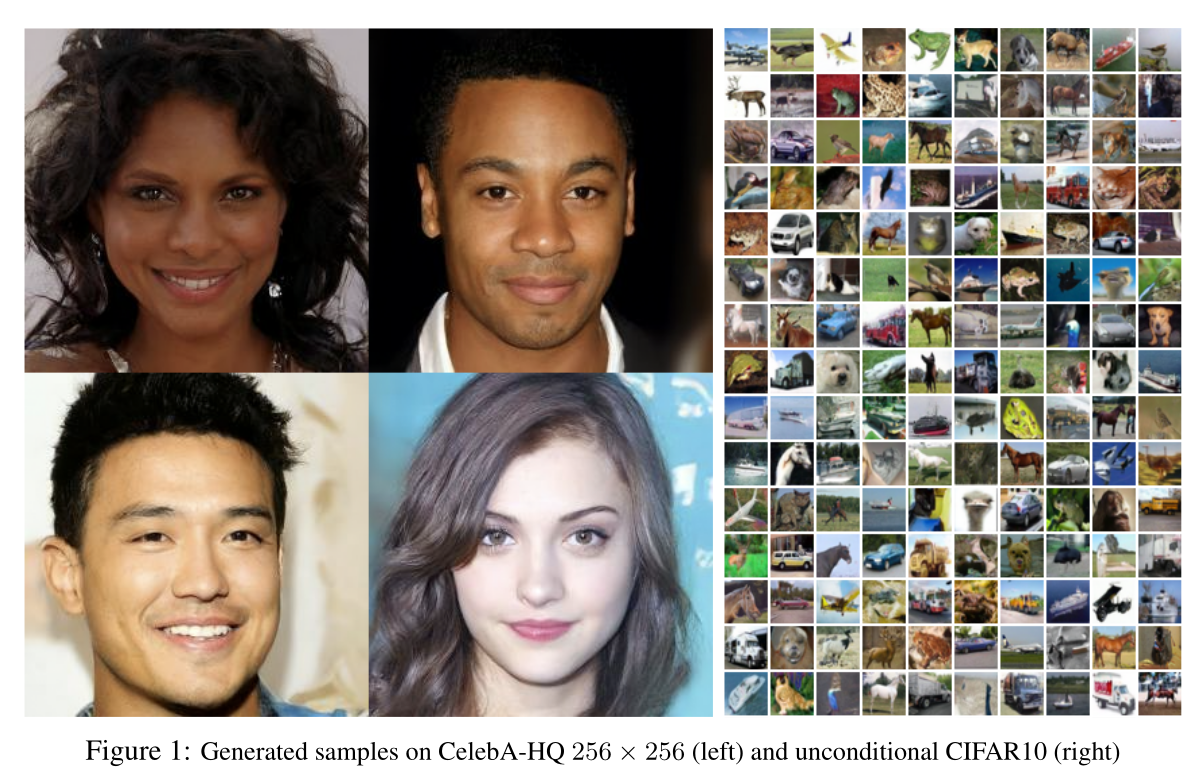
\includegraphics[width=0.6\textwidth]{figures/fake_faces.png}
    \caption{From \citep{ho2020denoising}.}
\end{figure}
\end{frame}

\begin{frame}
\frametitle{VAE Approach}
VAE \citep{kingma2013auto} makes some assumptions about family distribution to which $\mathcal{P}_{\mathcal{X}}$ belongs:
\begin{itemize}
    \item Existence of latent factors $\bm{z}$: $P(\bm{x}, \bm{z}) = P(\bm{x}\mid \bm{z}) P(\bm{z})$
    \item $P(\bm{x}|\bm{z}) = f_1(\bm{x}, \bm{z}; \boldsymbol \theta_1)$ where function class $f_1$ is some known distribution (in $\bm{x}$).
    \item $P(\bm{z}) = f_2(\bm{z}; \boldsymbol \theta_2)$ where function class $f_2$ is some known distribution (in $\bm{z}$).
\end{itemize}
Maximum likelihood principle suggests to maximize:
\[
\log P(\bm{x}) 
= \log \left( \sum_{\bm{z} \in \mathcal{Z}} P(\bm{x} \mid \bm{z}) P(\bm{z}) \right)
= \log \left( \sum_{\bm{z} \in \mathcal{Z}} f_1(\bm{x}, \bm{z}; \boldsymbol \theta_1) f_2(\bm{z}; \boldsymbol \theta_2) \right)
\] 
We can try to maximize its lower bound: For \textit{any} distribution $Q(\bm{z})$,
\[
\log P(\bm{x}) = 
\Dkl{Q(\bm{z})}{P(\bm{z} \mid \bm{x})}
+ \mathcal{L}(Q), \quad \text{where }
\mathcal{L}(Q) = \mathop{\mathbb{E}}_{\bm{z} \sim Q(\bm{z})} \left[ \log \dfrac{P(\bm{x}, \bm{z})}{Q(\bm{z})} \right]
\] 
Let $Q(\bm{z}) = f_3(\bm{z}; \boldsymbol \theta_3)$, and the lower bound can be maximized with respect to $\boldsymbol \theta_1, \boldsymbol \theta_2, \boldsymbol \theta_3$.

\begin{alertblock}{}
Could it be tractable without any assumption on $\mathcal{P}_{\mathcal{X}}$?
\end{alertblock}
\end{frame}

\begin{frame}
    \frametitle{Diffusion Model}
    Given an observed $\bm{x}_0 \sim \mathcal{P}_{\mathcal{X}}$, define a sequence of RVs $\bm{x}_1, \bm{x}_2, \ldots , \bm{x}_{T}$ \footnote{ abuse of notation}:
    \[
    \bm{x}_t = \sqrt{1- \beta_t} \bm{x}_{t-1} + \sqrt{\beta_t} \bm{z}_{t-1}, \quad t = 1, \ldots , T-1,
    \] 
    where 
    \begin{itemize}
        \item $\bm{z}_1, \ldots , \bm{z}_T$ are i.i.d, and $\bm{z}_t \sim \mathcal{N}(\bm{0}, \bm{I})$.
        \item $0 < \beta_0, \ldots , \beta_T < 1$ are predefined.
    \end{itemize}
    \begin{block}{Claims}
        \begin{enumerate}
            \item The sequence $\bm{x}_0, \ldots , \bm{x}_T$ satisfies Markov property: $P(\bm{x}_t \mid \bm{x}_{t-1}, \ldots , \bm{x}_0) = P(\bm{x}_t \mid \bm{x}_{t-1})$.
            \item If $T$ is large enough, $P(\bm{x}_T \mid \bm{x}_0)$ is approximately a Gaussian distribution \textit{regardless} of $\mathcal{P}_{\mathcal{X}}$.
            \item The backward direction of the chain also satisfies Markov property. In particular,
                \[
                \bm{x}_{t-1} = \left( 2- \sqrt{1 - \beta_{t+1}} \right) \bm{x}_t + \beta_t \nabla_{\bm{x}} \log p_t(\bm{x}_t) + \sqrt{\beta_{t+1}} \bm{z}_t
                \] 
        \end{enumerate}
    \end{block}
\end{frame}

\begin{frame}{Implication}
    \begin{block}{Claims}
        \begin{enumerate}
            \item The sequence $\bm{x}_0, \ldots , \bm{x}_T$ satisfies Markov property: $P(\bm{x}_t \mid \bm{x}_{t-1}, \ldots , \bm{x}_0) = P(\bm{x}_t \mid \bm{x}_{t-1})$.
            \item If $T$ is large enough, $P(\bm{x}_T \mid \bm{x}_0)$ is approximately a Gaussian distribution \textit{regardless} of $\mathcal{P}_{\mathcal{X}}$.
            \item The backward direction of the chain also satisfies Markov property. In particular,
                \[
                \bm{x}_{t-1} = \left( 2- \sqrt{1 - \beta_{t+1}} \right) \bm{x}_t + \beta_t \nabla_{\bm{x}} \log p_t(\bm{x}_t) + \sqrt{\beta_{t+1}} \bm{z}_t
                \] 
        \end{enumerate}
    \end{block}

    In VAE's world,
    \begin{itemize}
        \item Latent factor $\bm{z} = (\bm{x}_1, \ldots , \bm{x}_T)$
        \item Family of $P(\bm{z})$ is \textbf{well defined} without assumption,
            \[
            P(\bm{z}) 
            = \sum_{\bm{x}_0 \in \mathcal{X}} P(\bm{z}, \bm{x}_0) 
            = \sum_{\bm{x}_0 \in \mathcal{X}} \underbrace{P(\bm{x}_0 \mid \bm{x}_1)}_{\mathcal{N}(\boldsymbol \mu_1, \sigma_1^2 \bm{I})} \ldots \underbrace{P(\bm{x}_{T-1} \mid \bm{x}_T)}_{\mathcal{N}(\boldsymbol \mu_T, \sigma_T^2 \bm{I})} \, \underbrace{P(\bm{x}_T)}_{\mathcal{N}(\bm{0}, \bm{I})}
            \] 
        \item Family of $P(\bm{x} \mid \bm{z})$ is \textbf{well defined} without assumption,
        \[
        P(\bm{x} \mid \bm{z}) = P(\bm{x}_0 \mid \bm{x}_1, \ldots , \bm{x}_T) = P(\bm{x}_0 \mid \bm{x}_1)= \mathcal{N}(\boldsymbol \mu_1, \sigma_1^2 \bm{I})
        \] 
    \end{itemize}
    % The rest is just following VAE's recipe: find the lower bound, use reparameterization trick, \ldots 
\end{frame}

\begin{frame}
\frametitle{Proof of property 2} 

\begin{block}{Claims}
    \begin{itemize}
        \item If $T$ is large enough, $P(\bm{x}_T \mid \bm{x}_0)$ is approximately a Gaussian distribution \textit{regardless} of $\mathcal{P}_{\mathcal{X}}$.
    \end{itemize}
\end{block}
One step transition is
\[
P(\bm{x}_{i+1} \mid \bm{x}_{i}) \sim \mathcal{N}(\bm{x}_{i} \sqrt{(1-\beta_{i+1})} , \sqrt{\beta_{i+1}} \bm{I}),
\]
similarly, $t$ steps transition is
\[
P(\bm{x}_{i+t} \mid \bm{x}_i) 
= \mathcal{N}\left( \bm{x}_i \sqrt{\prod_{j=i+1}^{i+t}(1-\beta_j}) , \left(  1 - \prod_{j=i+1}^{i+t} (1-\beta_j)\right) \bm{I} \right),
\] 
Therefore, when $T$ is large enough,
\[
P(\bm{x}_T \mid \bm{x}_0) = 
\mathcal{N}\left( \bm{x}_0 \sqrt{\prod_{j=1}^{T}(1-\beta_j}) , \left(  1 - \prod_{j=1}^{T} (1-\beta_j)\right) \bm{I} \right) \quad \sim \quad \mathcal{N}(\bm{0}, \bm{I}),
\] 
\end{frame}
\begin{frame}
\frametitle{Define some constants} 
\[
P(\bm{x}_{i+t} \mid \bm{x}_i) 
= \mathcal{N}\left( \bm{x}_i \sqrt{\prod_{j=i+1}^{i+t}(1-\beta_j}) , \left(  1 - \prod_{j=i+1}^{i+t} (1-\beta_j)\right) \bm{I} \right),
\] 
Define some notation
\begin{align*}
&\alpha_t \triangleq 1- \beta_t, \\
&\overline{\alpha}_t = \prod_{s=1}^{t} \alpha_s
\end{align*}

\end{frame}
\begin{frame}{Proof of property 3}
\begin{itemize}
    \item $\bm{w}(t) \in \mathbb{R}^{d}$ is the standard Wiener process (or Brownian motion).

\end{itemize}
\begin{figure}
    \centering
    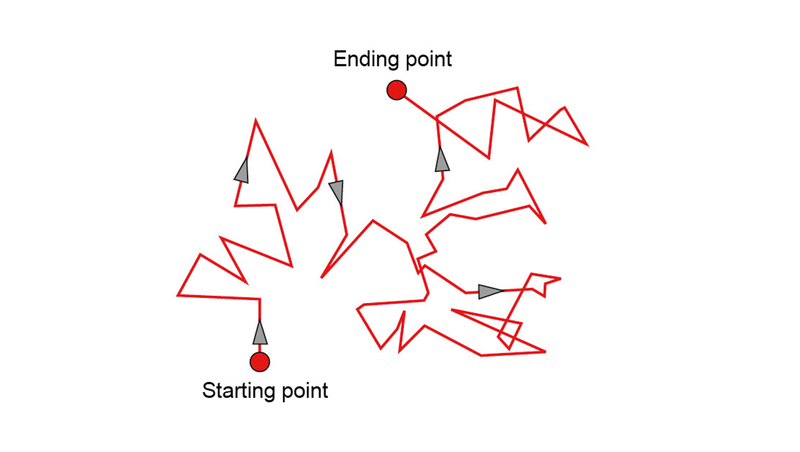
\includegraphics[width=0.7\textwidth]{figures/brownian.png}
    \caption{Brownian motion describes position of a random moving object, e.g., particles in water.}
\end{figure}
The increment $\bm{w}_{t_2} - \bm{w}_{t_1}$ is Gaussian with mean zero and variance $t_2 - t_1$.
\end{frame}

\begin{frame}{Informal proof of property 3}
\textit{Diffusion process.} Given
\begin{itemize}
    \item $\bm{x}(t): \mathbb{R}^{+} \to \mathbb{R}^{d}$ is a function of $t \geq 0$.
    \item $\bm{w}(t) \in \mathbb{R}^{d}$ is the standard Wiener process.
    \item $\bm{f}(\bm{x}, t): \mathbb{R}^{d} \times \mathbb{R} \to \mathbb{R}^{d}$: drift coefficient of $\bm{x}(t)$.
    \item $g(\cdot): \mathbb{R} \to \mathbb{R}$: diffusion coefficient of $\bm{x}(t)$.
\end{itemize}
then a diffusion process is governed by a stochastic differential equation (SDE)
\begin{subequations}
\label{eq:sde_forward}
\begin{align}
&x(0) \sim \mathcal{P}_{\bm{X}} \\
&d \bm{x} = \bm{f}(\bm{x}, t) dt + g(t) d \bm{w}
\end{align}
\end{subequations} 
By starting from samples of $\bm{x}_T \sim p_T$, and reverse process, we can obtain $\bm{x}(0) \sim \mathcal{P}_{\mathcal{X}}$.

Remarkable result from [x]: the reverse process is also a diffusion process, i.e, 
\begin{subequations}
\label{eq:sde_backward}    
\begin{align}
& \bm{x}(T) \sim p_T \\
&d \bm{x}(t) = \left( f(\bm{x}(t), t) - g(t)^2 \nabla_{\bm{x}} \log p_{t}(\bm{x}(t))\right)dt  + g(t)d \overline{\bm{w}},
\end{align} 
\end{subequations}
where $\overline{\bm{w}}$ is another standard Wiener process.
% A  to [x], the backward 
% A discretization version of the SDE above is
% \[
% \bm{x}_{t+1} - \bm{x}_{t} = \bm{f}_t(\bm{x}_t) + g_t \bm{z}_t, \quad \bm{z}_t \sim \mathcal{N}(\bm{0}, \bm{I})
% \] 
\end{frame}

\begin{frame}{Proof of property 3}
    Based on \fullcite{song2020score}.

\begin{proof}
\begin{itemize}
    \item Discrete the forward SDE $d \bm{x} = \bm{f}(\bm{x}, t) dt + g(t) d \bm{w} $:
\[
\bm{x}_{t+1} = \bm{x}_{t} + \bm{f}_{t}(\bm{x}) + g_t.
\] 
\item By choosing $ \bm{f}_t(\bm{x}) \triangleq \left(  \sqrt{1 - \beta_{t+1}}- 1\right) \bm{x}, \quad g_t \triangleq \sqrt{\beta_{t+1}}$, 
    \[
    \bm{x}_t = \sqrt{1- \beta_t} \bm{x}_{t-1} + \sqrt{\beta_t} \bm{z}_{t-1}, \quad t = 1, \ldots , T-1. \quad \text{(our original chain)}
    \] 
\item Discrete the backward SDE 
$ d \bm{x}(t) = \left( \bm{f}(\bm{x}(t), t) - g(t)^2 \nabla_{\bm{x}} \log p_{t}(\bm{x}(t))\right)dt  + g(t)d \overline{\bm{w}}$: 

\[
\bm{x}_{t-1} = \bm{x}_t - \bm{f}_t(\bm{x}_t) + g_t^2 \nabla_{\bm{x}} \log p_t(\bm{x}_t) + g_t\bm{z}_t.
\] 
\item Plug in $\bm{f}_t, g_t$:
\[
\bm{x}_{t-1} = (2 - \sqrt{1- \beta_{t+1}}) \bm{x}_{t} + \beta_{t+1} \nabla_{\bm{x}} \log p_t(\bm{x}_t) + \sqrt{\beta_{t+1}} \bm{z}_t
\] 
\end{itemize}
\end{proof}
\end{frame}

\begin{frame}{The SDE Framework}
Forward SDE
\[
d \bm{x} = \bm{f}(\bm{x}, t) dt + g(t) d \bm{w}
\] 
Backward SDE
\[
d \bm{x}(t) = \left( \bm{f}(\bm{x}(t), t) - g(t)^2 {\blue \nabla_{\bm{x}} \log p_{t}(\bm{x})} \right)dt  + g(t)d \overline{\bm{w}}
\] 
By choosing $\bm{f}(\bm{x}, t) ,g(t)$, we can design various diffusion process where $\bm{x}_T \sim p_T$ is in our control.

The remaining is to learn score function
\[
\boldsymbol \theta^{*} = \argmin_{\boldsymbol \theta} \mathop{\mathbb{E}}_{t} \left[ \lambda(t) \mathop{\mathbb{E}}_{\bm{x}(0)} \mathop{\mathbb{E}}_{\bm{x}(t) \mid \bm{x}(0)} \left[ \norm{\bm{s}_{\boldsymbol \theta}(\bm{x}(t), t) - \nabla_{\bm{x}(t)} \log p_{0t}(\bm{x}(t) \mid \bm{x}(0))}^2 \right]  \right]
\] 
\begin{itemize}
    \item Time $t$ is uniform sampled over $[0, T]$
    \item $\lambda(t): [0, T] \leftarrow \mathbb{R}^{+}$ is a weighting function
    \item $\bm{x}(0) \sim \mathcal{P}_{\mathcal{X}}$ and $\bm{x}(t) \sim P(\bm{x}(t) \mid \bm{x}(0))$ where $P(\bm{x}(t) \mid \bm{x}(0))$ is Gaussian if $\bm{f}(\bm{x}, t)$ is affine in $\bm{x}$.
    \item Expressiveness power of deep neural network is fully exploited here.
\end{itemize}
\end{frame}

\begin{frame}{The SDE Framework}
Forward SDE
\[
d \bm{x} = \bm{f}(\bm{x}, t) dt + g(t) d \bm{w}
\] 
Backward SDE
\[
d \bm{x}(t) = \left( \bm{f}(\bm{x}(t), t) - g(t)^2 {\blue \nabla_{\bm{x}} \log p_{t}(\bm{x})} \right)dt  + g(t)d \overline{\bm{w}}
\] 
Once $\bm{s}_{\boldsymbol \theta^{*}}(\bm{x}, t)$ is learned, we can derive the reverse diffusion process from the backward SDE
\[
d \bm{x}(t) = \left( \bm{f}(\bm{x}(t), t) - g(t)^2 {\blue \nabla_{\bm{x}} \log p_{t}(\bm{x})} \right)dt  + g(t)d \overline{\bm{w}}
\] 
and simulate it to sample $\bm{x}_0 \sim \mathcal{P}_{\mathcal{X}}$.
\begin{itemize}
    \item Solve the backward SDE using numerical SDE solver
    \item Ancestor sampling method \ldots 
\end{itemize}

The whole training and parameterization can be implemented under a probabilistic model, like in VAE.

\end{frame}

\begin{frame}{Training Process Under Probabilistic View}
Based on \fullcite{ho2020denoising}.
% This might be a boring part. But we have to cover it to see how people use diffusion in particular applications.

Define a generative model $\bm{x}_0 \leftarrow \bm{x}_1 \leftarrow \ldots  \leftarrow \bm{x}_T$ as
\begin{align}
&P(\bm{x}_T) \triangleq \mathcal{N}(\bm{0}, \bm{I}), \\
&P_{\boldsymbol \theta}(\bm{x}_0, \ldots , \bm{x}_T) \triangleq P(\bm{x}_T) \prod_{t=1}^{T} P_{\boldsymbol \theta}(\bm{x}_{t-1} \mid \bm{x}_t), \quad P(\bm{x}_{t-1} \mid \bm{x}_{t}) \triangleq \mathcal{N}(\boldsymbol \mu_{\boldsymbol \theta}(\bm{x}_t, t), \boldsymbol \Sigma_{\boldsymbol \theta}(\bm{x}_t, t)) \\
&P(\bm{x}_1, \ldots , \bm{x}_T \mid \bm{x}_0)  \triangleq \prod_{t=1}^{T} P(\bm{x}_t \mid \bm{x}_{t-1}), \quad P(\bm{x}_t \mid \bm{x}_{t-1}) \triangleq \mathcal{N}(\sqrt{1- \beta_t} \bm{x}_{t-1}, \beta, \bm{I})
\end{align}
With large $T$, there always exists $\boldsymbol \theta$ such that $\bm{x}_0 \sim \mathcal{P}_{\bm{X}}, \bm{x}_T \sim \mathcal{N}(\bm{0}, \bm{I})$.

How to perform inference on this model efficiently?
\end{frame}
\begin{frame}{Diffusion Model Inference}
    By maximum likelihood principle, we want to minimize
    \begin{align*}
    &\mathop{\mathbb{E}}_{\bm{x}_0 \sim P_{\boldsymbol \theta}(\bm{x}_0)} \left[ -\log P_{\boldsymbol \theta}(\bm{x}_0) \right] 
    \leq  
    \mathop{\mathbb{E}}_{P_{\boldsymbol \theta}(\bm{x}_0)} \left[ -\log P(\bm{x}_T) - \sum^{T}_{t=1} \log \dfrac{P_{\boldsymbol \theta}(\bm{x}_{t-1} \mid \bm{x}_t)}{P(\bm{x}_t \mid \bm{x}_{t-1})}\right] \\
    \quad \quad &= \mathop{\mathbb{E}}_{P_{\boldsymbol \theta}(\bm{x}_0)} \left[ \text{const} + \sum^{T}_{t>1} \underbrace{\Dkl{P(\bm{x}_{t-1} \mid \bm{x}_t, \bm{x}_0)}{P_{\boldsymbol \theta}(\bm{x}_{t-1} \mid \bm{x}_t)}}_{\blue L_{t-1}} - \text{almost const} \right],
    \end{align*} 
    This expression is better since $P(\bm{x}_{t-1} \mid \bm{x}_t, \bm{x}_0)$ is tractable, i.e.,
    \begin{align*}
    &P(\bm{x}_{t-1} \mid \bm{x}_t, \bm{x}_0) = \mathcal{N}(\bm{x}_{t-1}; \widetilde{\boldsymbol \mu}_t(\bm{x}_t, \bm{x}_0), \widetilde{\beta}_t \bm{I}), \\
    &\widetilde{\boldsymbol \mu}_t(\bm{x}_t, \bm{x}_0) \triangleq 
    \dfrac{\sqrt{\overline{\alpha}_{t-1} \beta_t}}{1- \overline{\alpha}_t} \bm{x}_0 + \dfrac{\sqrt{\alpha_t}(1- \overline{\alpha}_{t-1})}{1- \overline{\alpha}_t} \bm{x}_t
    \end{align*}

    We mostly only need to take care of ${\blue L_{t-1}}$ for $t=1, \ldots , T$. 

   The remaining part is how to parameterize 
    \[
    P_{\boldsymbol \theta}(\bm{x}_{t-1} \mid \bm{x}_t) = \mathcal{N}({\blue \boldsymbol \mu_{\boldsymbol \theta}(\bm{x}_t, t)}, \sigma_t^2 \bm{I})
    \] 
\end{frame}
\begin{frame}{Diffusion Model Inference}
    % Remaining part is to design parameterization of 
    % $ P_{\boldsymbol \theta}(\bm{x}_{t-1} \mid \bm{x}_t) = \mathcal{N}({\blue \boldsymbol \mu_{\boldsymbol \theta}(\bm{x}_t, t)}, \sigma_t^2 \bm{I})$.

    Recall that we want to minimize
    \begin{align*}
    L_{t-1} 
    &\triangleq \mathop{\mathbb{E}}_{\bm{x}_0 \sim P_{\boldsymbol \theta}(\bm{x}_0)} \left[\Dkl{P(\bm{x}_{t-1} \mid \bm{x}_t, \bm{x}_0)}{P_{\boldsymbol \theta}(\bm{x}_{t-1} \mid \bm{x}_t)} \right] \\
    &= \mathop{\mathbb{E}}_{\bm{x}_0 \sim P_{\boldsymbol \theta}(\bm{x}_0)} \left[ \dfrac{1}{2\sigma^2} \norm{\widetilde{\boldsymbol \mu}_t(\bm{x}_t, \bm{x}_0) - \boldsymbol \mu_{\boldsymbol \theta}(\bm{x}_t, t)}^2  \right] + C
    \end{align*} 
    Using reparameterization trick on $P(\bm{x}_t \mid \bm{x}_0) = \mathcal{N}(\sqrt{\overline{\alpha}_t} \bm{x}_0, (1-\overline{\alpha} \bm{I}))$,
    \[
    \bm{x}_t(\bm{x}_0, \boldsymbol \epsilon) = \sqrt{\overline{\alpha}_t} \bm{x}_0 + \sqrt{1- \overline{\alpha}_t} \boldsymbol \epsilon, \quad \boldsymbol \epsilon \sim \mathcal{N}(\bm{0}, \bm{I})
    \] 
    Plug in that $\bm{x}_t(\bm{x}_0, \epsilon)$,
    \[
    L_{t-1} - C = \mathop{\mathbb{E}}_{\bm{x}_0, \boldsymbol \epsilon} \left[ \dfrac{1}{2\sigma^2 }\norm{\dfrac{1}{\sqrt{\alpha_t}} \left( \bm{x}_t - \dfrac{\beta_t}{\sqrt{1-\overline{\alpha}_t}} \boldsymbol \epsilon \right) - \boldsymbol \mu_{\boldsymbol \theta}(\bm{x}_t, t)}^2 \right]
    \] 
    This clearly suggest a parameterization 
    \[
    \boldsymbol \mu_{\theta}(\bm{x}_t, t) \triangleq \dfrac{1}{\sqrt{\alpha_t}} \left( \bm{x}_t - \dfrac{\beta_t}{\sqrt{1-\overline{\alpha}_t}} \boldsymbol\epsilon_{\boldsymbol \theta}(\bm{x}_t, t) \right),
\]
where $\boldsymbol \epsilon_{\boldsymbol \theta}(\bm{x}_t, t)$ is neural network predicts true noise $\boldsymbol \epsilon$ from input $\bm{x}_t$ and time $t$.
\end{frame}
\begin{frame}{Diffusion Model Inference}
    Finally, the loss function would be
    \[
    \mathbb{E}_{\bm{x}_0, \boldsymbol \epsilon} \left[ \dfrac{\beta_t^2}{2\sigma^2_t \alpha_t(1- \overline{\alpha}_t)} \norm{\boldsymbol \epsilon - \boldsymbol \epsilon_{\boldsymbol \theta}(\sqrt{\overline{\alpha}_t} \bm{x}_0 + \sqrt{1-\overline{\alpha}_t} \boldsymbol \epsilon, t)}^2 \right]
    \] 
    And the sampling process is to sample recursively $\bm{x}_{t-1} \sim P_{\boldsymbol \theta}(\bm{x}_{t-1} \mid \bm{x}_t)$,
    \[
    \bm{x}_{t-1} = \dfrac{1}{\sqrt{\alpha_t}} \left( \bm{x}_t - \dfrac{\beta_t}{\sqrt{1- \overline{\alpha}_t}} \boldsymbol \epsilon_{\boldsymbol \theta}(\bm{x}_t, t) \right)
    \] 

\end{frame}

\begin{frame}{Take home points}
\begin{itemize}
    \item Expressively powerful as there is almost no assumption about family of $\mathcal{P}_{\mathcal{X}}$ while being \textbf{tractable}.
    \item Error occurs in choosing $T$, choosing function class of score function $\bm{s}_{\boldsymbol \theta}$, learning $\bm{s}_{\boldsymbol \theta}$
    \item No assumption about input structure (vs VAE): 1d, 2d\ldots , image, text, \ldots. 
\end{itemize}
\end{frame}

\begin{frame}{Diffusion Model in Action.}
    \begin{itemize}
        \item High resolution image generation.
        \item Conditional generative model.
        \item Inverse problem.
    \end{itemize}
\end{frame}

\begin{frame}{Applications: High resolution image generation}
    \fullcite{rombach2022high}.
    This paper is the core of Stable Diffusion.

    Diffusion process on image space is too expensive. 
    \begin{itemize}
        \item Find a good latent space, a good encoder $\mathcal{E}$ and decoder $\mathcal{D}$
        \item Project all data to this latent space $\bm{z}_i = \mathcal{E}(\bm{x}_i) \sim \mathcal{P}_{\mathcal{Z}}$
        \item Run diffusion to sample new latent vector $\bm{z} \sim \mathcal{P}_{\mathcal{Z}}$
        \item Decode the latent vector to get new image $\mathcal{D}(\bm{z})$
    \end{itemize}
\end{frame}

\begin{frame}{Conditional generation setting.}
    Setting:
    \begin{itemize}
        \item We have a list of paired data $(\bm{x}_1, \bm{y}_1), (\bm{x}_2, \bm{y}_2), \ldots , (\bm{x}_N, \bm{y}_N)$ where $\bm{y}_i$ is additional information about $\bm{x}_i$, such as class label, text describing the image.
        \item Later, we want to sample new $\bm{x}$ given particular $\bm{y}$.
    \end{itemize}
Define a generative model $\bm{x}_0 \leftarrow \bm{x}_1 \leftarrow \ldots  \leftarrow \bm{x}_T$ as
\begin{align}
&P(\bm{x}_T \mid \bm{y}) \triangleq \mathcal{N}(\bm{0}, \bm{I}), 
P_{\boldsymbol \theta}(\bm{x}_0, \ldots , \bm{x}_T \mid \bm{y}) \triangleq P(\bm{x}_T \mid \bm{y}) \prod_{t=1}^{T} P_{\boldsymbol \theta}(\bm{x}_{t-1} \mid \bm{x}_t, \bm{y}), \\
&P(\bm{x}_{t-1} \mid \bm{x}_{t}, \bm{y}) \triangleq \mathcal{N}(\boldsymbol \mu_{\boldsymbol \theta}(\bm{x}_t, t, \bm{y}), \boldsymbol \Sigma_{\boldsymbol \theta}(\bm{x}_t, t, \bm{y})) \\
&P(\bm{x}_1, \ldots , \bm{x}_T \mid \bm{x}_0, \bm{y})  \triangleq \prod_{t=1}^{T} P(\bm{x}_t \mid \bm{x}_{t-1}, \bm{y}), \quad P(\bm{x}_t \mid \bm{x}_{t-1}, \bm{y}) \triangleq \mathcal{N}(\sqrt{1- \beta_t} \bm{x}_{t-1}, \beta, \bm{I})
\end{align}
The loss function would be
    \[
    \mathbb{E}_{\bm{x}_0, \bm{y}, \boldsymbol \epsilon} \left[ \dfrac{\beta_t^2}{2\sigma^2_t \alpha_t(1- \overline{\alpha}_t)} \norm{\boldsymbol \epsilon - \boldsymbol \epsilon_{\boldsymbol \theta}(\sqrt{\overline{\alpha}_t} \bm{x}_0 + \sqrt{1-\overline{\alpha}_t} \boldsymbol \epsilon, t, \bm{y})}^2 \right]
    \] 

\end{frame}

\begin{frame}{Applications: Image Restoration}
\fullcite{wang2022zero}

Given 
\[
\bm{y} = \bm{A} \bm{x} + \bm{n},
\] 
where $\bm{y}$ is observed signal, $\bm{A}$ is known linear operator (dow-sampling of an image, sampling matrix in compressed sensing, \ldots ), $\bm{x}$ is the original signal that we wish to recover, $\bm{n}$ is nonlinear noise.

Existing approaches are
\begin{itemize}
\item Domain knowledge-based regularization
        \[
\widehat{\bm{x}} = \argmin_{\bm{x}} \dfrac{1}{2} \sum^{N}_{i=1} \norm{\bm{y}_i - \bm{A}\bm{x}_i}^2 + \lambda \mathcal{R}(\bm{x}_i)
\] 
% where $\mathcal{R}(\bm{x})$ is regularization term used to promote some prior knowledge about $\bm{x}$. For example, if $\bm{x}$ is an clean image, it should not change very much from pixel to pixel, hence the use of total variance as a regularizer. If $\bm{x}$ is a signal in compressed sensing setting, it might be sparse, hence the use of l1 norm. 
\item Then deep learning comes in: data distribution-based regularization
\[
\argmin_{\bm{w}} \norm{\bm{A} \mathcal{G}(\bm{w}) - \bm{y}}^2 + \lambda \mathcal{R}(\bm{w}),
\] 
\end{itemize}
\end{frame}
\begin{frame}
Solution of $\bm{y} = \bm{A}\bm{x}$ is
\[
    \widehat{\bm{x}} = \bm{A}^{\dagger} \bm{y} + (\bm{I} - \bm{A}^{\dagger} \bm{A}) \overline{\bm{x}}, \quad \; \forall  \overline{\bm{x}}
\] 
So the idea is to find $\overline{\bm{x}}$ such that $P(\widehat{\bm{x}}; \overline{\bm{x}}) = \mathcal{P}_{\mathcal{X}}$.

In order to do so, and note that the requirement of \textit{data consistency} is only required on $\bm{x}_0$, not all the other $\bm{x}_i$'s (during the sampling process).
\begin{itemize}
    \item Sample $\bm{x}_T$
    \item Sample $\bm{x}_{t-1}$ based on $\bm{x}_t$
    \item Infer $\bm{x}_0$ from $\bm{x}_t$
    \item Rectify $\bm{x}_0$ to get $\widehat{\bm{x}}_0$ such that $\bm{A} \widehat{\bm{x}_0} = \bm{y}$ (so it satisfies data consistency)
    \item Get the ``rectify'' version of $\bm{x}_{t-1}$, namely $\widehat{\bm{x}}_{t-1}$
    \item Back to step 2
\end{itemize}
\end{frame}
\begin{frame}{In details}
    Recall that
    \[
        \bm{x}_t(\bm{x}_0, \boldsymbol \epsilon) = \sqrt{\overline{\alpha}_t} \bm{x}_0 + \sqrt{1- \overline{\alpha}_t} \boldsymbol \epsilon, \quad \boldsymbol \epsilon \sim \mathcal{N}(\bm{0}, \bm{I})
    \] 
    Suppose we have $\bm{x}_t$,
    a good trained diffusion model gives us 
    $\boldsymbol \epsilon_{\widehat{\boldsymbol \theta}}(\bm{x}_t, t) \approx \boldsymbol \epsilon$, then an estimate of $\bm{x}_0$ given $\bm{x}_t$ is
    \[
\widehat{\bm{x}}_{0 \mid t} = \dfrac{1}{\sqrt{\overline{\alpha}_t}} \left( \bm{x}_t - \boldsymbol \epsilon_{\widehat{\boldsymbol \theta}}(\bm{x}_t, t) \sqrt{1-\overline{\alpha}_t} \right)
    \] 
    Modify this to satisfy data consistency,
    \[
    \widetilde{\bm{x}}_{0\mid t} = \bm{A}^{\dagger} \bm{A} \bm{y} + (\bm{I} - \bm{A}^{\dagger} \bm{A}) \widehat{\bm{x}}_{0\mid t}
    \] 
    Then we can sample $\bm{x}_{t-1}$ as $\bm{x}_{t-1} \sim P(\bm{x}_{t-1} \mid \bm{x}_{t}, \widetilde{\bm{x}}_{0 \mid t})$,
    \[
    \bm{x}_{t-1} = \dfrac{\sqrt{\overline{\alpha}_{t-1}} \beta_t}{1-\overline{\alpha}_t} \widetilde{\bm{x}}_{0\mid t} + \dfrac{\sqrt{\alpha_t}(1- \overline{\alpha}_{t-1})}{1-\alpha_t}\bm{x}_t + \sigma_t \boldsymbol \epsilon  , \quad \boldsymbol \epsilon \sim \mathcal{N}(\bm{0}, \bm{I})
    \] 
\end{frame}
\begin{frame}
    Some thoughts
    \begin{itemize}
        \item We only need to train diffusion model once, and then freeze it.
        \item But we need to know linear operator $\bm{A}$ in advance
    \end{itemize}
\end{frame}

% \begin{frame}{Application: }
% \fullcite{graikos2022diffusion}
%
% Task: Inferring $\bm{x}$ given $c(\bm{x}, \bm{y})$ where $\bm{y}$ is some observed information, and also given $p(\bm{x})$ (bald). This general description includes the image restoration problem in the previous section.
% \end{frame}

\begin{frame}{Something else}
    \begin{itemize}
        \item \fullcite{carlini2023extracting}
        \item And measure performance of generative model is still a controversial topic
        \item Energy-based models.
        \item Discrete latent.
    \end{itemize}
\end{frame}

\end{document}
